\chapter{Experiments and Analysis}

\section{Environment}
All the code for this algorithm was written in Python and Rust. Python was used to read and sanitize the initial dataset, and Rust was used to generate the binary purchase vectors. We opted to use Rust instead of Python for this task because the generation of this vectors has a time complexity of $O(N^2)$ at worst, and therefore may take an order of magnitude longer to run on a slower language such as Python. Python was used for the rest of the tasks, which included the graph generation and clustering, as well as the itemset generation and rule pruning. The following external Python libraries were used to aid development:
\begin{itemize}
\item \texttt{pandas}: Data manipulation.
\item \texttt{numpy}: Data manipulation.
\item \texttt{matplotlib}: Plotting library.
\item \texttt{seaborn}: Plotting library.
\item \texttt{networkx}: Graph generation and plotting.
\item \texttt{markov\_clustering}: Markov Clustering Algorithm.
\end{itemize}

\section{\algo\ and Apriori Algorithm}
We used both the \algo\ and the Apriori Algorithm to generate rules for our dataset, with the support constraint at $0.1\%$ and the confidence constraint at $25\%$. Given these constraints, the Apriori algorithm generated $1,222$ rules, and the \algo\ generated $123$ bi-cluster rules as well as $40$ intra-cluster rules, totalling $163$ rules.\\
\\\\\textbf{Apriori Rules}\\
We present the first 5 rules generated by the Apriori Algorithm, ranked by highest support.\\
\texttt{\{chewing gum and candy\} $\rightarrow$ \{cigarettes\}}\\\texttt{support: 0.0726 | confidence: 0.2986 | lift: 1.0985}\\
\texttt{\{cigarettes\} $\rightarrow$ \{chewing gum and candy\}}\\\texttt{support: 0.0726 | confidence: 0.2671 | lift: 1.0985}\\
\texttt{\{water\} $\rightarrow$ \{chewing gum and candy\}}\\\texttt{support: 0.0473 | confidence: 0.3052 | lift: 1.2554}\\
\texttt{\{filters\} $\rightarrow$ \{lubricant\}}\\\texttt{support: 0.0468 | confidence: 0.9381 | lift: 2.6850}\\
\texttt{\{chocolates\} $\rightarrow$ \{chewing gum and candy\}}\\\texttt{support: 0.0435 | confidence: 0.3117 | lift: 1.2820}\\
\\\textbf{\algo}\\
Similarly, we present the first 5 rules generated by the \algo, ranked by highest support. The type of rule has also been annotated (i.e. bi-cluster or intra-cluster).\\
\texttt{\{chewing gum and candy\} $\rightarrow$ \{cigarettes\}}\\\texttt{support: 0.0726 | confidence: 0.2986 | lift: 1.0985 | type: bi-cluster}\\
\texttt{\{cigarettes\} $\rightarrow$ \{chewing gum and candy\}}\\\texttt{support: 0.0726 | confidence: 0.2671 | lift: 1.0985 | type: bi-cluster}\\
\texttt{\{water\} $\rightarrow$ \{chewing gum and candy\}}\\\texttt{support: 0.0473 | confidence: 0.3052 | lift: 1.2554 | type: intra-cluster}\\
\texttt{\{filters\} $\rightarrow$ \{lubricant\}}\\\texttt{support: 0.0468 | confidence: 0.9381 | lift: 2.6850 | type: intra-cluster}\\
\texttt{\{chocolates\} $\rightarrow$ \{chewing gum and candy\}}\\\texttt{support: 0.0435 | confidence: 0.3117 | lift: 1.2820 | type: bi-cluster}\\
\\\textbf{Analysis}\\
We observe that there is a $100\%$ overlap between the top five rules generated by the Apriori algorithm and the \algo. The $100\%$ overlap stands true for up until the first $13$ rules for both algorithms. 
\begin{figure}[H]
\centering
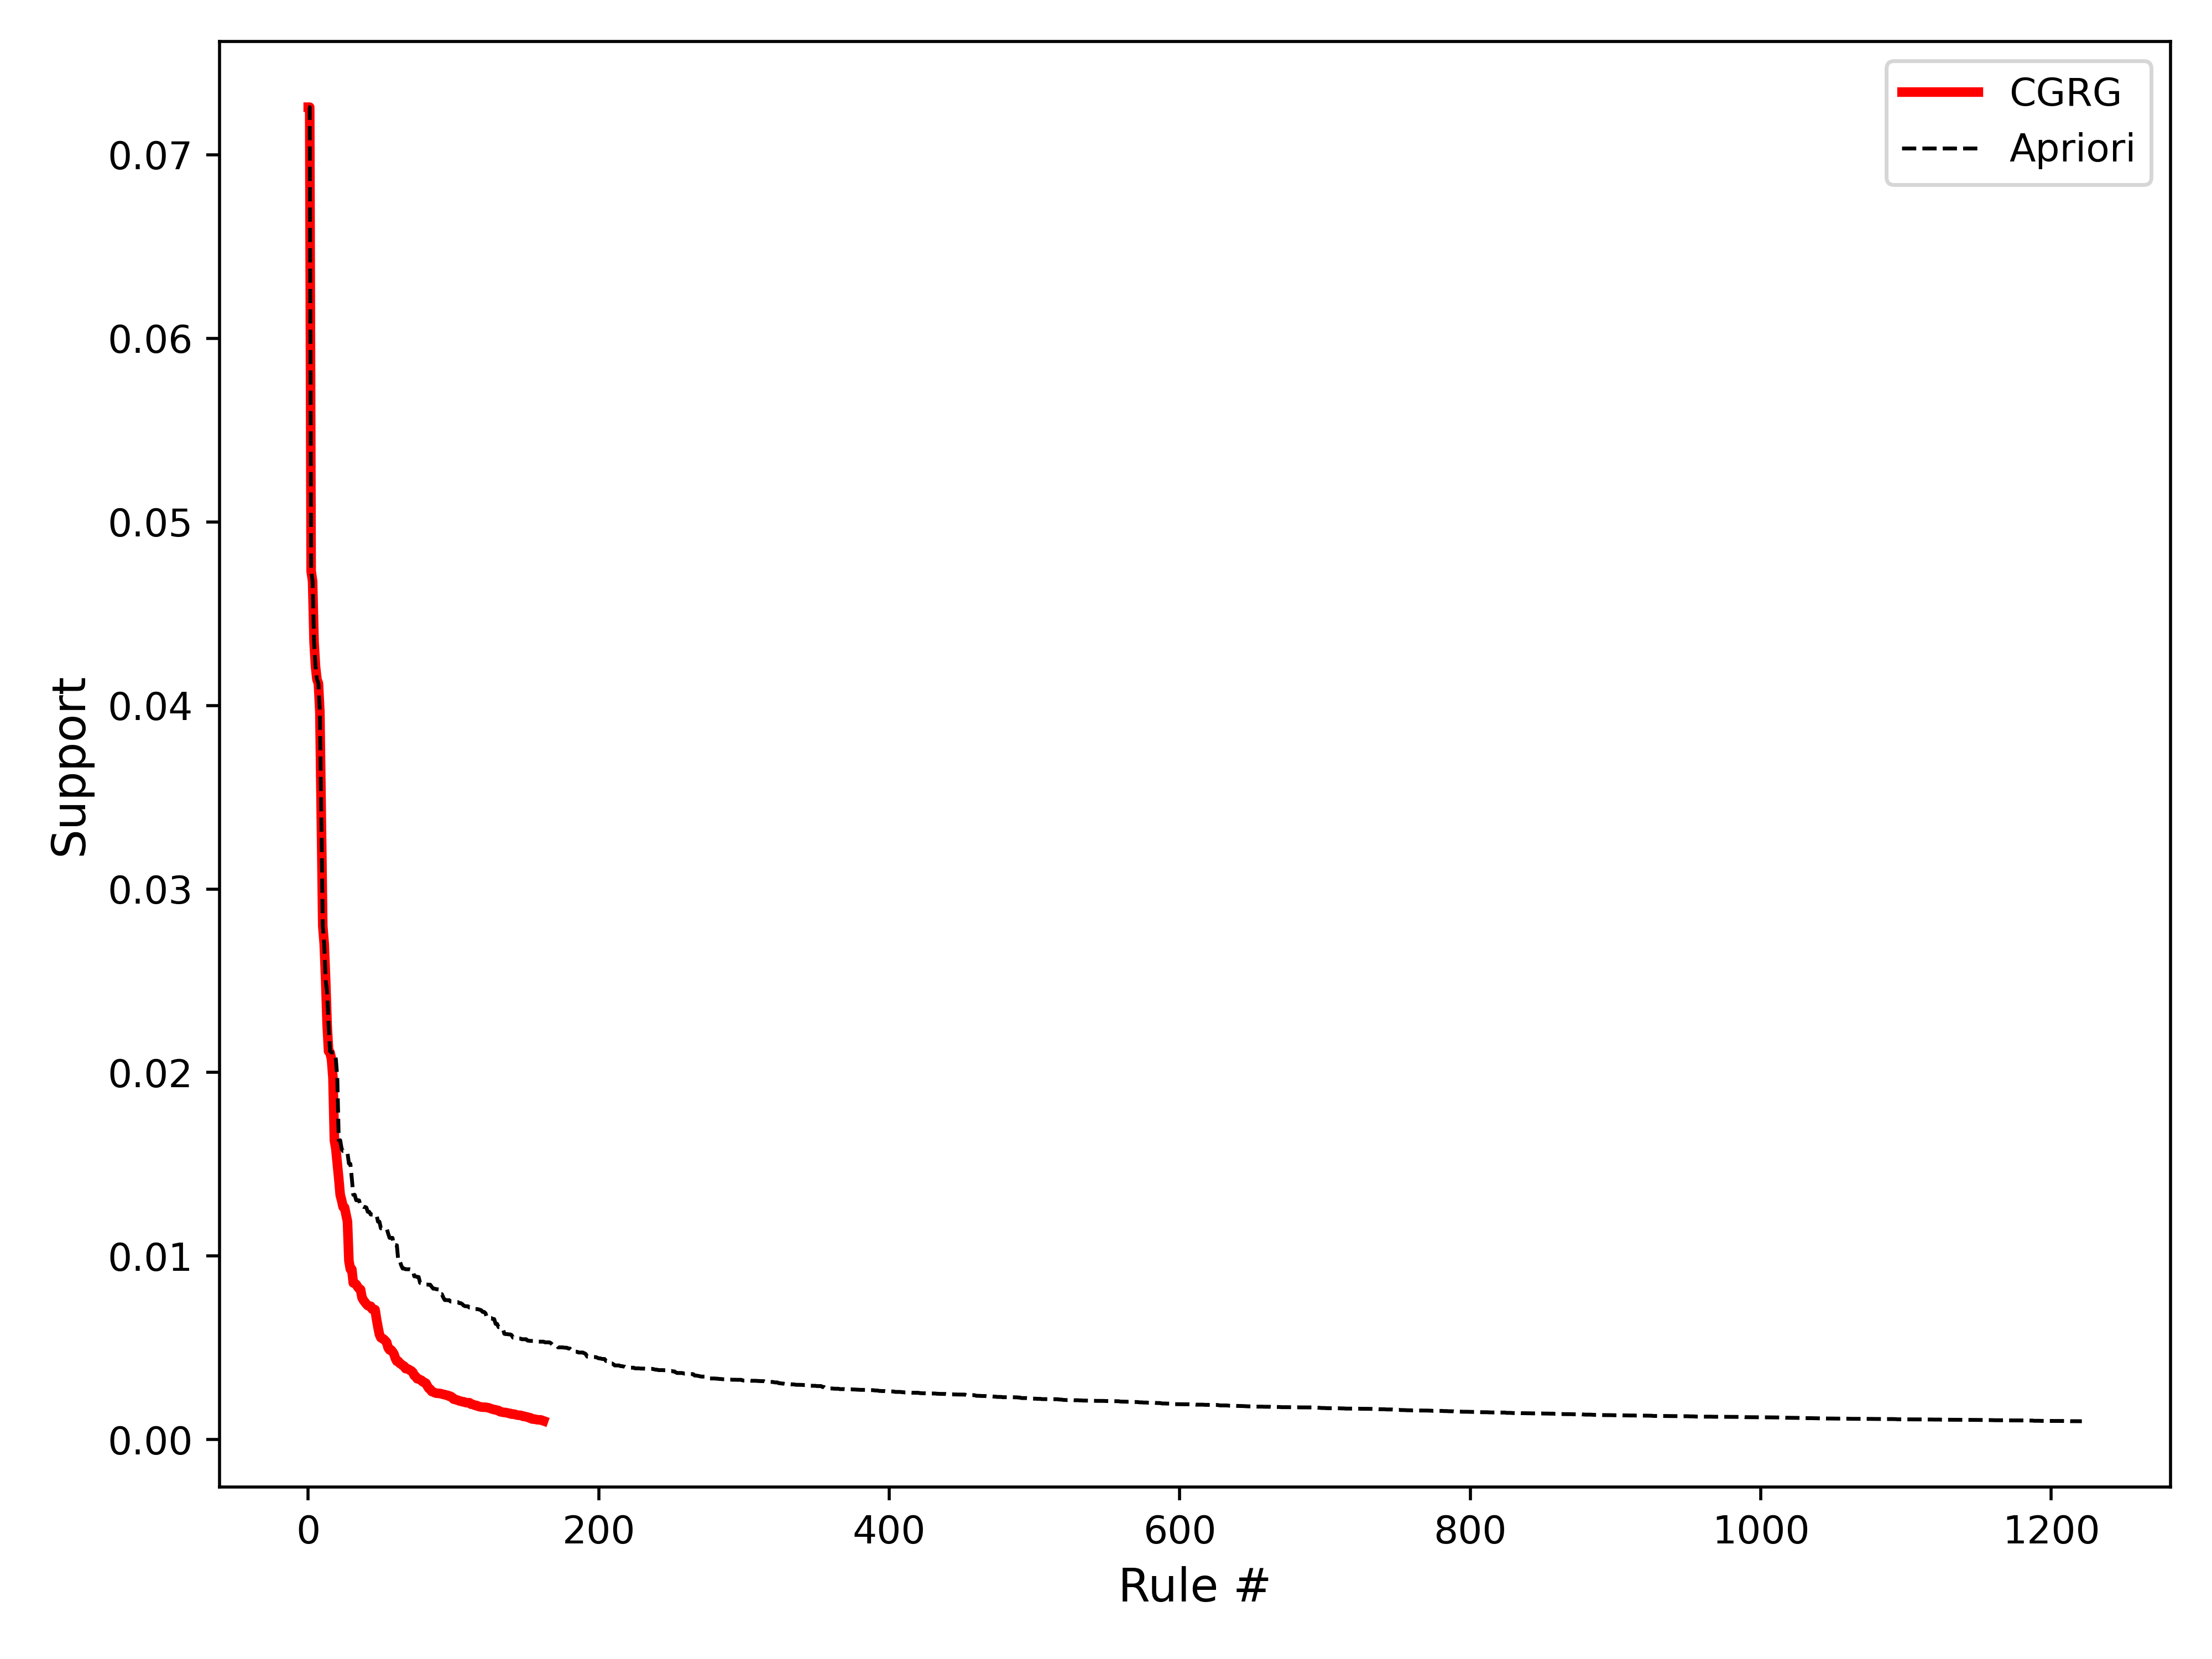
\includegraphics[scale=0.65]{ruleset_support}
\caption{Ranked supports for both the \algo\ and Apriori Algorithm}
\label{fig:rule_support}
\end{figure}
Figure \ref{fig:rule_support} illustrates the support values for the $x^{th}$ rule for both the \algo\ and Apriori when they are sorted by highest support score to lowest. We can infer from this figure that the \algo\ captures the strongest rules present in the Apriori ruleset, which leads us to another conclusion: \textit{describe rule here}. In other words, given an itemset $I = i_1,i_2,\dots,i_m$ and clusters $A$ and $B$, rules which follow:
\[
i_k \rightarrow i_j
\]
\[
i_k \subset A, \;\;\; (i_j \subset B \;|\; i_j \subset A)
\]
are more likely to have a higher support score than rules whose antecedent and/or consequent are composed of items from multiple clusters.